\section{Detector performance}

In order to calibrate detectors and test their performances, a cosmic test bench was designed and installed at Saclay early in the project (Figure \ref{fig:mm-testbench}). The goal of these tests is to determine the best operating conditions of a detector and to compute its 2D efficiency map using cosmic muons.


\begin{figure}[htb]
 \missingfigure[figwidth=6cm]{Saclay test bench}
 \caption{Cosmic bench made of an external trigger from the coincidence of two scintillators and a hodoscope made of 4 reference trackers. The picture shows the operation of a Barrel and a Forward detector simultaneously under test.}
 \label{fig:mm-testbench}
\end{figure}

The cosmic test bench shown on Figure, consists of a vertical stack of six detectors. Two scintillators are installed at the top and the bottom of the stack to provide the trigger. Four $50 \times 50 \text{cm}^2$ double-layers flat Micromegas are used as a tracker to provide the reference track of a cosmic ray. In the middle of the stack, empty trays receive the detectors which must be characterized.

After alignment of the reference trackers and the detectors in test, the efficiency is measured in few days by comparing the reference track provided with the signals collected on the test Micromegas tile or disk. All MVT detectors have been systematically characterized before shipment to JLab. These tests included a study of the efficiency as a function of the amplification voltage and a two-dimensional efficiency map.

The results were similar for all detectors: the efficiency plateau starts at about 500V with a value between 98.5\% and 99.5\% at 510V. It was shown that the plateau was slightly shifted to higher strip voltages when the drift plane is at higher voltage because the mesh loses electron transparency. The 2D-efficiency map was useful to look for any structural problem. All MVT detectors that were shipped to Jefferson Lab had uniform 2D-efficiency map. And example of the efficiency plateau and the the 2D efficiency map is shown in Figure \ref{fig:mm-fig8}.

\begin{figure}[htb]
 \missingfigure[figwidth=6cm]{efficiency plateau and 2D map}
 \caption{Efficiency plateau (left) and 2D map (right) for a C-type barrel detector.}
 \label{fig:mm-fig8}
\end{figure}

\subsection{Commissioning}

The Micromegas vertex tracker was delivered in June 2017 at JLab. A Saclay team of 10 people assembled the MVT and combined it with the SVT to form the final configuration of the CLAS12 central vertex tracker.  The MVT barrel was first commissioned with cosmic rays in a gray room until mid-October and for the first two weeks once installed in the Hall. The final phase of the commissioning started in December 2017 with beam. Before describing the results of the different commissioning phases, one should mention some difficulties during this critical period:

\begin{itemize}
 \item Even though Saclay was responsible for the distribution of gas to the detectors, Jefferson Lab was responsible for providing the adequate gas mixture. Due to US budget issues, this gas mixing system has only been completed mid-March 2018, more than 9 months after the target delivery date. Because Jefferson Lab could not buy enough premix gas bottles due to budget restrictions, the commissioning with cosmic rays had to be limited to the bare minimum in order to spare enough gas to take some commissioning data with beam. It is only since mid-February 2018 that Micromegas are being operated in steady conditions, i.e. with a continuous flow of gas.
 
 \item Jefferson Lab was also responsible for the central tracking software (SVT+MVT). During the first phase of commissioning with beam, it appeared that the SVT suffered from unplanned radiation damage which had dire consequences for the S/N ratio. Unfortunately, the tracking code turned out to have little flexibility and was hardwired to start looking for tracklets with only the SVT (which had a very large single-hit multiplicity). The tracking in its initial form was therefore very inefficient which made it difficult for us to get immediate result. We immediately reacted by taking in charge the modification of the tracking algorithm, but significant progress was only obtained recently. The other consequence of this issue, is that without a good way of measuring the tracking efficiency of our detectors, we essentially ran blind during this first beam phase, as far as HV settings were concerned. In addition, very little to no work was done by the Jefferson Lab software team on using FMT in the forward tracking algorithm. Once again, this made it quite hard both to understand and to operate the detector.

\end{itemize}

\subsubsection{Central Vertex Tracker commissioning with cosmic rays}

Although integrated in June 2017, the commissioning of the Central Vertex Tracker with cosmic rays has started late August 2017. Indeed, due to budget restrictions, Jefferson Lab could only provide a limited number of premix gas bottles necessary for Micromegas operation. 

Most of the work focused on electronics (data taking, noise study), slow controls (remote controls access and interlocks), gas system tests, and detector tests. A faulty FEU and splitter for optical fibers were found. Translation tables, geometry and tracking codes were fine-tuned with the first cosmic rays. 

A second commissioning period ran from late September to mid-October 2017. This period was dedicated mostly to tuning detector settings and understanding detector data. The first task was to locate the efficiency plateau, which was found to be 20V higher than in Saclay due to a different gas mixture: the 90-10 mixture in the premix bottle is a volumetric ratio, whereas in Saclay the mixture was based on the mass of the compounds. Once settings were adjusted, cosmic-ray data were collected for alignment purposes. The alignment could not be performed as soon as the cosmic data were collected, considering the higher priority set to the implementation of a monitoring tool for beam commissioning and the on-going installation in the Hall. This monitoring tool has been the cornerstone of the commissioning: its purpose was to provide fast feedback for all Micromegas detectors in order to quickly find the basic settings to collect data, such as the latency with respect to the trigger, HV settings, etc. A screenshot of this tool is shown on Figure \ref{fig:mm-fig10}. It was used to spot in a timely manner the reason of any issue or quantify any improvement during the fine-tuning of the initial settings.

\begin{figure}[htb]
 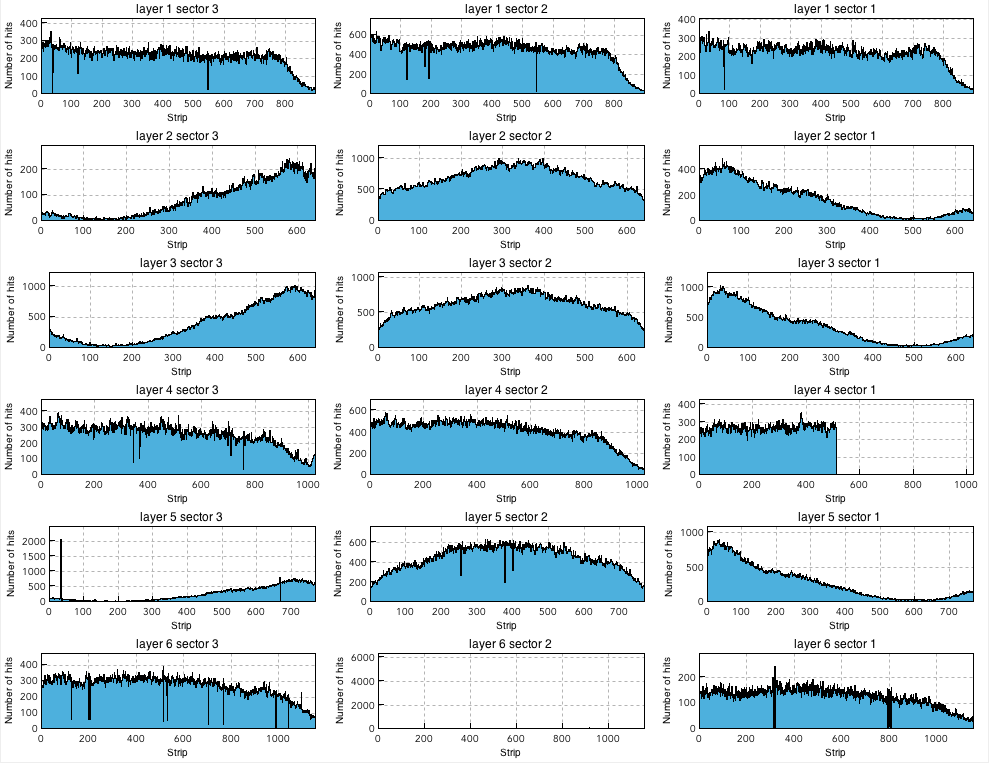
\includegraphics[width=.45\textwidth]{images/fig10}
 \caption{Hit occupancies of a cosmic-ray run with the trigger delivered by the SVT. Layers 1, 4 and 6 are C-tiles. Layers 2, 3 and 5 are Z-tiles. Since the SVT is shorter than the barrel, it does not provide trigger for the downstream part of the C-tiles (high strip numbers). The sector 2 of the barrel covers the SVT whereas the sector 1 and 3 are covering mostly the side of the SVT. The missing half tile of layer 4 sector 1 is due to the faulty FEU. The layer 6 was replaced a few weeks later, early September..}
 \label{fig:mm-fig10}
\end{figure}

Finally, a third and last period of commissioning with cosmic rays started in the Hall once the CVT was inserted inside the solenoid magnet. Thanks to the common noise subtraction, the noise levels were found as low as in the gray room despite all the possible sources of noise present in the Hall such as solenoid fields, surrounding pumps and electronic equipment. Unlike in the gray room, the CTOF provided the trigger and its acceptance was large enough to cover the first disks of FMT, which we turned on. 

As previously stated, all Micromegas detectors used premix gas. Unfortunately, we could only run 1/3 of the time to keep gas for beam commissioning. Also, we used the same Argon-isobutane mixture for both the FMT and BMT, which was not planned: FMT was supposed to use a ternary mix of Argon-Isobutane-CF


\subsubsection{Central Vertex Tracker commissioning with beam}

As with any new detector, the commissioning with beam was performed progressively and carefully. As long as the beam was not stable, the MVT HVs were off. At first, all current limits on the HV were set to 0.5$\mu$A in order to protect the detectors. For both BMT and FMT, the HVs have been slowly increased until they would reach the nominal settings. During empty target runs and/or with beam currents less than 20nA, nominal HV values were reached for both strips and drift HV. However, at nominal luminosity ($10^{35}\text{cm}^{-2}\text{s}^{-1}$), the charge collected onto the strips itself induces a current higher than the 0.5$\mu$A. Indeed, as shown in Figure \ref{fig:mm-fig14}, the current on the strips is about 1.75 $\mu$A at nominal luminosity on the strips for the barrel (75nA on 5cm-long target of liquid hydrogen). Limits on strips have then been increased accordingly.

\begin{figure}[htb]
 \missingfigure[figwidth=6cm]{Currents vs beam current}
 \caption{Currents on the strips as a function of beam current on full target. All detectors have similar currents. The nominal luminosity of $10^{35}\text{cm}^{-2}\text{s}^{-1}$ corresponds to 75nA on our 5cm-long LH2 target.}
 \label{fig:mm-fig14}
\end{figure}

The next step was to find the efficiency plateau with beam and 5T magnetic field. As of today, the tracking algorithm is not efficient enough to do such a study with BMT and FMT. Since no absolute efficiency could be derived in a timely manner, the cluster multiplicity per electron trigger was studied instead, as shown on Figure \ref{fig:mm-fig15}. Indeed, this observable was found to get flatter where the efficiency plateau was expected to be from the commissioning with cosmic rays.  For the FMT, the plateau was found from 460V to 490V. Above 490V, the cluster multiplicity and the current on the strips increase suddenly. It was decided to set 460V as nominal HV settings for FMT, which allows safe operations with a 75nA beam. The Corona effect seems to occur around 540V in the barrel and the nominal HV setting was decided to be 520V.  Occupancies are about 3.5\% for the FMT disks and 2.5\% for the BMT tiles at nominal luminosity, as shown on Figure \ref{fig:mm-fig16}.


\begin{figure}[htb]
 \missingfigure[figwidth=6cm]{Cluster multiplicity in FMT vs HV}
 \caption{Cluster multiplicity in FMT as a function of HV on the strips.}
 \label{fig:mm-fig15}
\end{figure}


\begin{figure}[htb]
 \missingfigure[figwidth=6cm]{Occupancy vs beam current}
 \caption{Occupancies of FMT (left) and BMT (right) as a function of the beam current. Half of the FMT disks has a lower occupancy since only their inner region is active.}
 \label{fig:mm-fig16}
\end{figure}

The commissioning resumed on January 12th.  The second commissioning period was performed with different beam energies: 2.2, 6.4 and 10.6GeV. At 2.2GeV, the recoil proton from elastic scattering could be seen in the hit occupancies of the C-detector without any tracking, as shown on Figure 17. A typical event in the central detectors at 10.6GeV beam energy is shown on Figure 18. One can see the high occupancy in the SVT detectors making the MVT mandatory for high efficiency tracking in this background condition.



\section{Readout performance}

The summer-fall cosmic ray commissioning phase and the December 2017 engineering run validated the functionality of the MVT readout system. The slow control of the front-end electronics was integrated within the overall CLAS12 EPICS framework. Continuous monitoring of temperatures, on-board generated voltages and power consumption were possible for each of the 48 FEUs as well as for entire readout system. Implemented software interlocks preventing overheating and overcurrent of the frontends proved itself efficient.

According to field maps the residual magnetic field of the 5T solenoid may vary from 0.6T to 0.8T in the MVT frontend electronics area. It had no apparent influence on the readout system performance. During several ramp-up and ramp-down sessions of the magnet no detectable increase of the overall power consumption or of the supply currents of individual FEU were detected. The data acquisition was stable as well.

The cosmic ray commissioning permitted finalizing of the MVT acquisition software integration with the CLAS12 CODA framework. A suite of utilities was developed to perform automated runs to determine the pedestal equalization parameters and zero suppression thresholds for data taking, in addition to a quick analysis of the MVT data quality estimation and timing adjustment.

The low (about 20 Hz) trigger rate of the cosmic runs allowed to keep a relatively large number of samples for each retained channel with the charge deposition above the programmed zero suppression threshold. 16 samples proved enough to encompass completely the detector signals giving the possibility to perform detector performance studies. However, the luxury to keep the entire shape of the signals is not possible during the beam operation. Indeed, with the trigger rates as high as 10 kHz the CLAS12 event builder throughput will not be enough to absorb the total amount of data produced by MVT. The number of samples was reduced to 6 in accordance to the design specifications. The readout timing window with the retained samples was centered on the signals' maxima. Two modes of operation were used: consecutive and sparse readouts, as shown on Figure 19. The first one implies the readout of consecutive samples. With the sampling rate of 25 MHz, the timing window is $6 \times 40 = 240 \text{ns}$ wide. The sparse mode was set to readout every other sample (equivalent to a 80 ns period) resulting to the doubled timing window of 480 ns with wider signal shape recorded.


Even with this optimization, the average archived MVT data per event of about 13 Kbyte remained higher than the estimated 6 Kbyte used for the design specifications. At 10 kHz trigger rate the so-called EVIO formatted data throughput exceeded the bandwidth of the single 1 GB Ethernet link connecting the unique MVT backend to the CLAS12 event builder network. The raw non-formatted data exchanged between the two SSP/BEU modules and the crate controller was saturating the 200 Mbyte/s throughput of the VME backplane. Despite of the bottlenecks, the built-in rate regulation capabilities made the MVT system operate stably at about 7.5 kHz max trigger rate imposing dead-time on the CLAS12 DAQ. 

Both bottlenecks were removed in January 2018 by splitting the single backend in two backend crates. During the following physics run, trigger rates of 10-12 kHz were sustained routinely. Recently further improvement was performed by installing 10 GB Ethernet network interface cards on the controllers of the both backend crates. This will allow trigger rates of 20 kHz foreseen for the physics run during the fall 2018.

Nevertheless, the difference between the projected MVT event size and the observed one has to be understood. The influence of the ambient electro-magnetic noise can be excluded as the vast majority of the collected data contains well-shaped detector signals. The data reduction starts to be significant when the zero suppression thresholds are above 8σ of common-mode corrected pedestal noise, cutting drastically down the number of retained channels with otherwise good signal content.

Even if the large data volume turns out to be inherent to operation of the MVT detectors in the high current beam, further improvement of sustainable trigger rates is possible. If the studies will indicate an acceptable signal timing “walk”, one can a) envisage diminishing the number of samples to 5 reducing both the background and physics generated data; and b) diminishing the zero-suppression window from the current 120 ns to 80 ns reducing the contribution from the ghost hits generated by the background. An obvious performance improvement would be the distribution of the backend functionality from the two to three crates lessening the burden on the VME backplane. About 50 kHz trigger rate can be envisaged. The above improvements do not require any additional developments and are already supported by the current hardware, firmware and software. Two further modifications are viable but require development efforts of varying intensity. Firstly, one can double the bus width within the SSP/BEU firmware increasing the processing and formatting of the FEU packets in order to perform the local event building faster. Lastly, one can replace the current signal distribution module in the backend by the JLAB VXS-Trigger-Processor and use its 10/40 GB Ethernet port as the interface with the event builder thus avoiding completely the VME bus. This ultimate change would allow the use of single backend crate. Trigger rates as high as 65 kHz can be expected and even higher (80 kHz if 4-sample readout is acceptable).
